Self-organized criticality can be studied through cellular automata. The specific CA studied in this project is the \emph{sandpile} model, first introduced by Bak, Tang, and Wiesenfeld (BTW) in 1987 \cite{bak1987self}. While in two dimensions, the analogy to a physical sandpile can theoretically be made, we view a sandpile as an abstract $d$-dimensional CA as defined below. The definitions and the method for simulating and analyzing sandpiles in this project largely follow the 1991 paper by Christensen et al. \cite{christensen1991dynamical}.

%%%%%%%%%%%%%%%%%%%%%%%%%%%%%%%%%%%%%%%%%%%%%%%%%%%%%%%%%%%%%%%%%%%%%%%%%%%%%%%%%%%%%%%%
\subsection{The BTW sandpile automaton}
%%%%%%%%%%%%%%%%%%%%%%%%%%%%%%%%%%%%%%%%%%%%%%%%%%%%%%%%%%%%%%%%%%%%%%%%%%%%%%%%%%%%%%%%

\begin{figure}
    \centering
    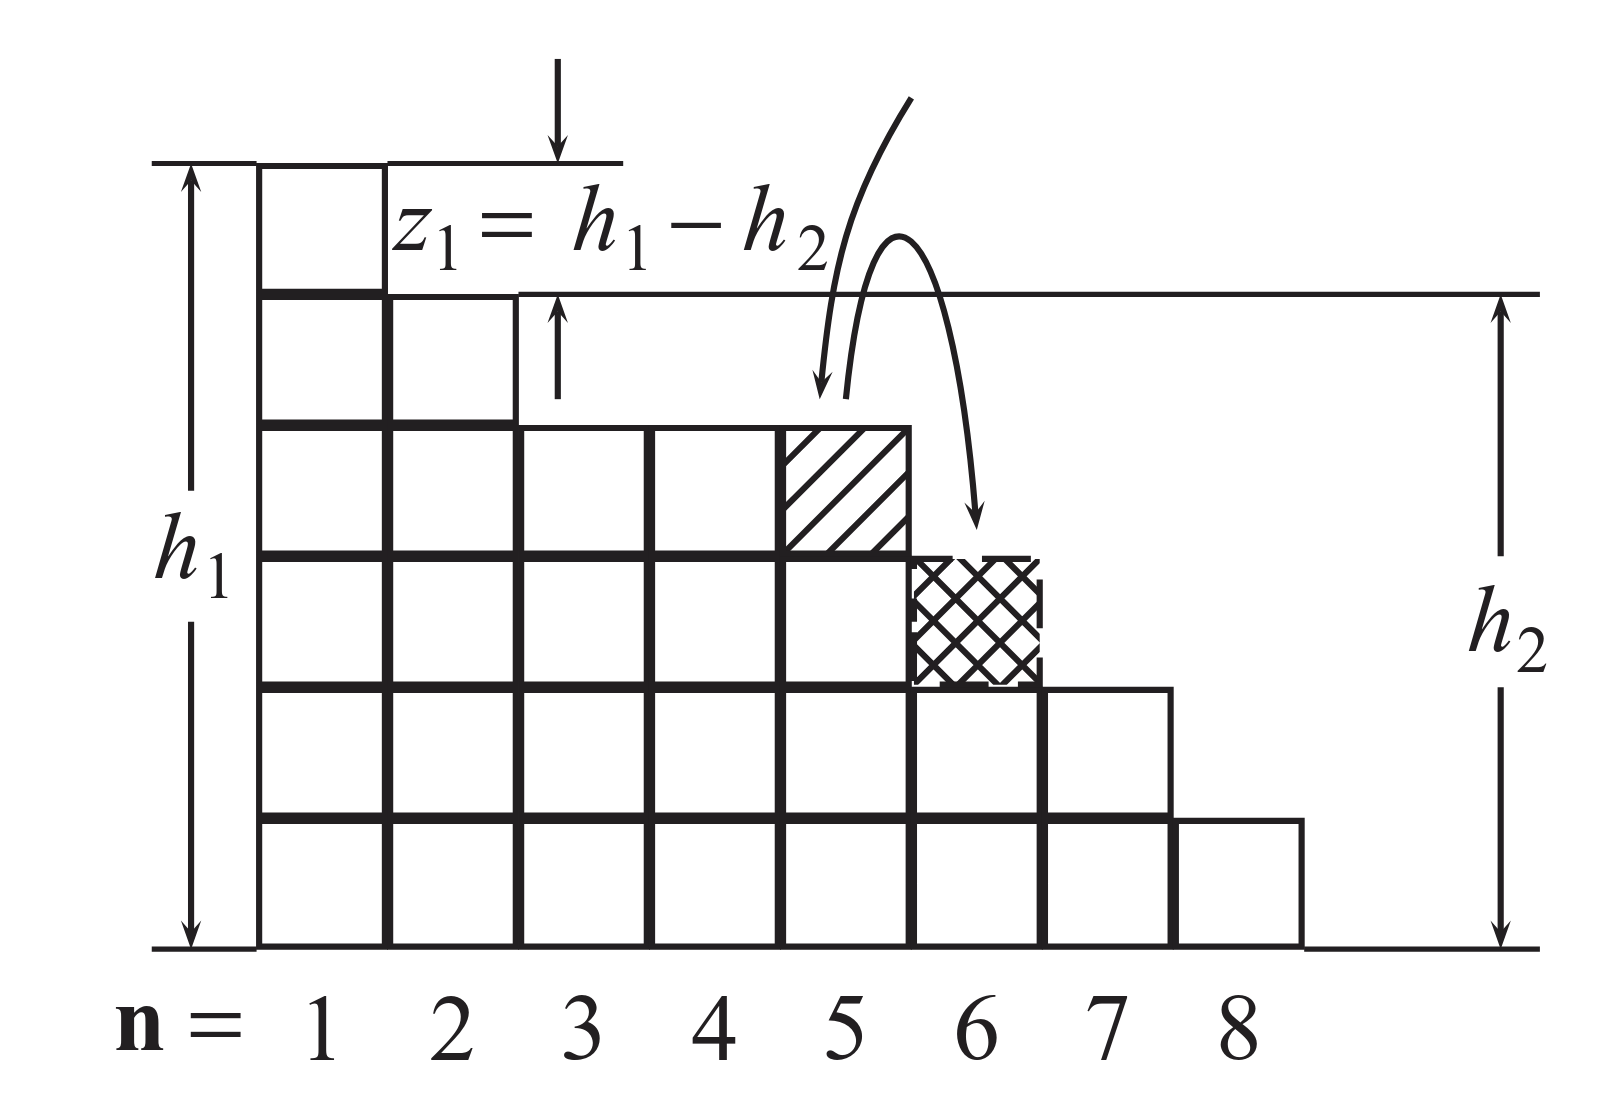
\includegraphics[width=0.8\linewidth]{../../figures/local_slope.png}
    \caption{This illustration shows in a one-dimensional example, how the configuration $z(r)$ can be interpreted as the local slope of a sandpile with heights $h$ on the vertices between the lattice sites. Source: Pruessner 2012, Chapter 4.1 \cite{pruessner2012self}.}
    \label{fig:local-slope}
\end{figure}

A sandpile of dimension $d$ and linear size $N$ is defined on the lattice
\begin{equation}
    R := (\bN_{\leq N})^d \subseteq \bZ^d.
\end{equation}
The neighborhood $M_r$ of a lattice site $r\in R$ is defined as the set of the site itself and all directly adjacent lattice sites
\begin{equation}
    M_r := \{r\} \cap \{r \pm e_i \mid 1\leq i\leq d\},
\end{equation}
where $e_i$ is the lattice's $i$-th canonical unit vector. The configuration $z$ assigns an integer $z_\tau(r)\in\bZ$ to each lattice site $r$ at time $\tau$. Christensen et al. \cite{christensen1991dynamical} call this configuration the \emph{local slope} of the sandpile at time $\tau$, which is motivated by the physical analogy shown in Figure \ref{fig:local-slope}. Another, perhaps more universal, way is to think of $z$ as the \emph{local energy} of the system at a lattice site \cite{barrat1999fluctuations},\cite{markovic2014power}. We shall from now on stick to this analogy. Next, we define a critical threshold $z_c\in\bZ$. The sandpile is \emph{stable}, if at a given time step, $z(r) \leq z_c$ for all $r\in R$. Otherwise, the system is \emph{unstable}. The time evolution of the sandpile is then specified as follows.

If the sandpile is stable, the local evolution leaves $z$ constant, i.e. $z_{\tau+1}(r) = z_\tau(r)$ for all $r$. Hence, without changing $z$ through an external perturbation, a stable sandpile does not change in time at all. For an unstable sandpile, let
\begin{equation}
    R_u(\tau) := \{r\in R \mid z_\tau(r) > z_c\}
\end{equation}
be the set of all unstable sites. Then at each unstable lattice site a \emph{toppling} event occurs, which dissipates one unit of energy from the unstable site to each of its $2d$ direct neighbors. The time evolution $\tau\to\tau+1$ thus reads
\begin{align}
    z_\tau(r) &\to z_\tau(r) - 2d, \label{eqn:relaxation} \\
    z_\tau(r\pm e_i) &\to z_\tau(r\pm e_i) + 1 \qq{for} i=1,\ldots,d \nonumber
\end{align}
for all $r\in R_u(\tau)$. The time evolution step of an unstable sandpile is also called \emph{relaxation} and all topplings happen simultaneously at every unstable lattice site.

Inside the lattice, relaxation events preserve the total energy
\begin{equation}
    z_\mathrm{tot} = \sum_{r\in R}z(r)
\end{equation}
of the system, as can be seen from Equation (\ref{eqn:relaxation}). Only at the lattice boundaries, where $r_i=1$ or $r_i=N$ for some $1\leq i\leq N$, can the energy be dissipated.

%%%%%%%%%%%%%%%%%%%%%%%%%%%%%%%%%%%%%%%%%%%%%%%%%%%%%%%%%%%%%%%%%%%%%%%%%%%%%%%%%%%%%%%%
\subsection{Boundary conditions}
%%%%%%%%%%%%%%%%%%%%%%%%%%%%%%%%%%%%%%%%%%%%%%%%%%%%%%%%%%%%%%%%%%%%%%%%%%%%%%%%%%%%%%%%

Following \cite{christensen1991dynamical}, we consider two kinds of boundary conditions. In \emph{open} boundary conditions, the relaxation step is modified to
\begin{align}
    z_\tau(r) &\to z_\tau(r) - 2d + (\text{number of }i\text{ with }r_i=N), \nonumber \\
    z_\tau(r+e_i) &\to z_\tau(r+e_i) + 1 \qq{if} r_i\neq N, \\
    z_\tau(r-e_i) &\to z_\tau(r-e_i) + 1 \qq{for} i=1,\ldots,d, \nonumber \\
\intertext{and}
    z_\tau(r) &= 0 \qq{if} r_i=1 \text{ for any i}. \nonumber
\end{align}
Furthermore, we define closed boundary conditions by enforcing
\begin{equation}
    z_\tau(r) = 0 \qq{if} r_i=1\text{ or } r_i=N \text{ for any i}.
\end{equation}
Note that our lattice coordinates run from $1$ to $N$, hence $r_i=1$ forms the lower boundary.

After a certain amount of relaxation steps, an unstable sandpile reaches a stable state through dissipation at the lattice boundaries. A consecutive number of $t$ relaxations which brings an unstable sandpile to a stable state is called an \emph{avalanche} of lifetime $t$.

%%%%%%%%%%%%%%%%%%%%%%%%%%%%%%%%%%%%%%%%%%%%%%%%%%%%%%%%%%%%%%%%%%%%%%%%%%%%%%%%%%%%%%%%
\subsection{Perturbations}
%%%%%%%%%%%%%%%%%%%%%%%%%%%%%%%%%%%%%%%%%%%%%%%%%%%%%%%%%%%%%%%%%%%%%%%%%%%%%%%%%%%%%%%%

In order to observe criticality, we must introduce an external perturbation that changes the configuration $z$ of the sandpile. Christensen et al. \cite{christensen1991dynamical} define two types of perturbations. A \emph{conservative} perturbation of a lattice site $r_0$ given by
\begin{align}
    z(r_0) &\to z(r_0) + d, \label{eqn:con_perturb} \\
    z(r_0-e_i) &\to z(r_0-e_i) - 1 \qq{for} i=1,\ldots,d
\end{align}
keeps the total energy of the system constant (except for the lower boundaries), while a \emph{nonconservative} perturbation
\begin{equation}
    z(r_0) \to z(r_0) + 1 \label{eqn:noncon_perturb}
\end{equation}
adds a unit of energy to a random point on the sandpile.

The model studied in this work considers perturbations in the slow driving limit, which means that perturbation and relaxation happen on different time scales \cite{barrat1999fluctuations}. This means that the system is allowed to fully relax before the next perturbation is introduced. Hence, the perturbations happen on a macroscopic time scale, detached from the relaxation steps, which are the microscopic evolution of the CA.

%%%%%%%%%%%%%%%%%%%%%%%%%%%%%%%%%%%%%%%%%%%%%%%%%%%%%%%%%%%%%%%%%%%%%%%%%%%%%%%%%%%%%%%%
\subsection{The critical state} \label{sec:critical-state}
%%%%%%%%%%%%%%%%%%%%%%%%%%%%%%%%%%%%%%%%%%%%%%%%%%%%%%%%%%%%%%%%%%%%%%%%%%%%%%%%%%%%%%%%

After a transient period of $T$ macroscopic time steps, which we also call \emph{burn-in} phase, all sandpiles, except for the closed system with conservative perturbation, reach a stationary state. The burn-in time $T$ depends on the initial configuration of the system as well as the chosen boundary conditions and perturbations \cite{christensen1991dynamical}. In the stationary state, which we also call critical state, the average energy
\begin{equation}
    \expval{z}(\tau) = \frac{1}{\abs{R}}\sum_{r\in R}z_\tau(r) \label{eqn:z_mean}
\end{equation}
fluctuates around a temporal mean value
\begin{equation}
    \overline{\expval{z}} = \lim_{T'\to\infty}\frac{1}{T'-T}\int_{T}^{T'}\expval{z}(\tau)\dd{\tau}.
\end{equation}
This means that in this state, the energy introduced to the sandpile by each perturbation averages out with the energy lost through avalanches by dissipation at the boundaries over time. Once a sandpile has reached a critical state, it remains in this state \cite{gros2015cellular}. Hence the term Self-Organized Criticality \cite{Dhar1990}.

In the stationary state, spatial correlations in the system extend over all length scales and the system lacks any intrinsic length or time scale \cite{pruessner2012scaling}. As mentioned in Section \ref{sec:power-laws}, this leads to the emergence of power laws in the probability densities of certain avalanche observables.

%%%%%%%%%%%%%%%%%%%%%%%%%%%%%%%%%%%%%%%%%%%%%%%%%%%%%%%%%%%%%%%%%%%%%%%%%%%%%%%%%%%%%%%%
\subsection{Avalanche variables}
%%%%%%%%%%%%%%%%%%%%%%%%%%%%%%%%%%%%%%%%%%%%%%%%%%%%%%%%%%%%%%%%%%%%%%%%%%%%%%%%%%%%%%%%

Christensen et al. \cite{christensen1991dynamical} propose three avalanche characteristics, which are random variables that can be measured. Let $\tau=0$ be the time step at which an avalanche starts after a perturbation at $r_0\in R$. Then the lifetime $t$ of the avalanche is the total number of microscopic time steps it takes for the sandpile to reach a stable state,
\begin{equation}
    t = \min\{\tau\geq0 \mid R_u(\tau) = \emptyset\}.
\end{equation}
The total size $s$ of the avalanche is defined as the cumulative sum of the number of toppling events, i.e. the number of unstable lattice sites, that happen during each relaxation step
\begin{equation}
    s = \sum_{\tau=0}^t \abs{R_u(\tau)}.
\end{equation}
The linear size $l$ of the avalanche is the maximum coordinate distance from the perturbation center to any point that is affected by the avalanche
\begin{equation}
    l = \max_{0\leq\tau\leq t}\{\norm{r_0-r_u}_\infty \mid r\in R_u(\tau)\}.
\end{equation}
When the system is in a critical state, we expect the behavior of avalanche characteristics to obey power laws. For the probability densities of the random variables, they are typically defined as
\begin{align}
    P(T=t) &\propto t^{1-\alpha}, \nonumber \\
    P(S=s) &\propto s^{1-\tau}, \label{eqn:pdfs} \\
    P(L=l) &\propto l^{1-\lambda}, \nonumber
\end{align}
where $\alpha,\tau,\lambda$ are scaling parameters to be determined. Note that the parameter $\tau$ here is different from the timestep $\tau$ used before. Additionally, we also expect the conditional expectation values of the avalanche parameters with respect to each other to obey the power laws
\begin{align}
    \bE[S \mid T=t] &\propto t^{\gamma_1}, \nonumber \\
    \bE[T \mid S=s] &\propto s^{1/\gamma_1}, \nonumber \\
    \bE[S \mid L=l] &\propto l^{\gamma_2}, \nonumber \\
    \bE[L \mid S=s] &\propto s^{1/\gamma_2}, \label{eqn:expvals} \\
    \bE[T \mid L=l] &\propto l^{\gamma_3}, \nonumber \\
    \bE[L \mid T=t] &\propto t^{1/\gamma_3}. \nonumber
\end{align}
In the following, we want to perform numerical measurements and validate the emergence of power laws by statistically measuring the probability densities (Eq. (\ref{eqn:pdfs})) and expectation values (Eq. (\ref{eqn:expvals})) and calculate the respective scaling exponents.
